\documentclass{article}
\usepackage{parskip}
\usepackage{pdfpages}
\usepackage{hyperref}
\usepackage{amsmath}
\usepackage[margin=.6in]{geometry}
\begin{document}
\includepdf[pages=3]{slides}
\includepdf[pages=4]{slides}
There is set of rules that make up the knowledge base of the system (describe it logically)

We have a set of if-then rules which we amalgamate using fuzzy reasoning so that we can derive an inference (aka decision signal).

\includepdf[pages=5]{slides}
We have a cylindrical extension C  to find the cylinder that will intersect with f to create the antecedent. P is the projection on the compliment universe of discourse. When we apply this to our antecedent we get B, our second fuzzy set. f is the set of knowledge about the rules between A and B. We need the fuzzy set A to be 3d to match f so that we can do the intersection which is why we apply C to it.

\includepdf[pages=7]{slides}
a -> fuzzy relation f on x and y.  if x is the temperature and y is the level of the air conditioner, then this is the result.

b -> cylindrical extension of a, basically $C(A)$

c -> this is just p  this is the result of $C(A)\cap f$

d -> projection of (c) onto y, this is also just the max of the relationship in c and put it over y, also known as the consequent

\includepdf[pages=6]{slides}
So B is the max over all x's of the min of the cylindrical extension of x and the relationship between x and y.

So its using the max-min composition rule

This is just the simplest case we are dealing with one variable in antecedent and one variable at consequent


\includepdf[pages=8]{slides}
\includepdf[pages=9]{slides}
\includepdf[pages=10]{slides}
\includepdf[pages=11]{slides}
Using the associativity level we put together all the sets in the same universe of discourse, A and A'. B belongs to the compliment universe of discourse so it stays on its own. The t-norm is the linking value between A and A'. We call the degree of validity, the common region between A and A' and quantify it by the value given as level. This is then mapped to the compliment. The result of this gives us the membership function for B'.

The highest value of intersection of A and A' to get the weight, then map this onto the membershipt of B to get the consequent.

This is known as the mamdani representation for inferencing (aka min T-norm).

\includepdf[pages=12]{slides}
Now we move on to multiple variables. For example we have temperature an humidity to deal with.

You do exactly the same thing (if you only have one rule) and just take the minimum value for them. This lowest value is called the firing strength.

\includepdf[pages=13]{slides}
\includepdf[pages=14]{slides}
\includepdf[pages=15]{slides}

































\end{document}
